\section{Results}
\label{sec:04-results}

\subsection{Qualitative results}

To show the results of global motion estimation it is easier to use some qualitative information, also because the reader will understand it straightforwardly.

One of the applications that shows inuitively the implications of global motion estimation is camera motion compensation. 
Basically, if the video is recorded by a camera which is moving, we will see the two types of motion explained in \cref{sec:01-intro}: apparent and real. The aim of camera-motion compensation is to detect and remove the (apparent) motion which is caused only by the (ego)motion of the camera.

To show the results obtained we reported in image \red{qualitative-result-image} an example in which the reader can observe:
\begin{itemize}
    \item first row position 1, the previous frame;
    \item first row position 2, the next frame;
    \item first row position 3, the compensated frame;
    \item second row position 1, the absolute difference between next and previous frame;
    \item second row position 2, the motion field generated by the camera as returned by our estimation procedure;
    \item second row position 3, the absolute difference between the next frame and the compensated one.
\end{itemize}

\begin{figure*}[htbp]
    \begin{subfigure}[b]{0.3\textwidth}
        \centering
        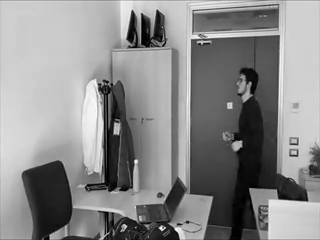
\includegraphics[width=1\textwidth]{../assets/images/04-prev-frame.png}
        \caption{Previous frame}
        \label{fig:prev-frame}
    \end{subfigure}
    \hfill
    \begin{subfigure}[b]{0.3\textwidth}
        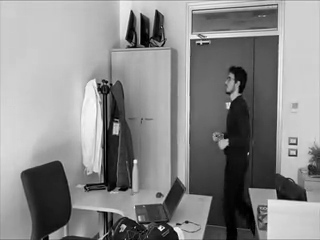
\includegraphics[width=1\textwidth]{../assets/images/04-curr-frame.png}
        \caption{Previous frame}
        \label{fig:curr-frame}
    \end{subfigure}
    \hfill
    \begin{subfigure}[b]{0.3\textwidth}
        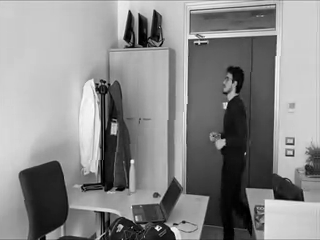
\includegraphics[width=1\textwidth]{../assets/images/04-compensated.png}
        \caption{Compensated frame}
        \label{fig:compensated}
    \end{subfigure}
    
    \begin{subfigure}[b]{0.3\textwidth}
        \centering
        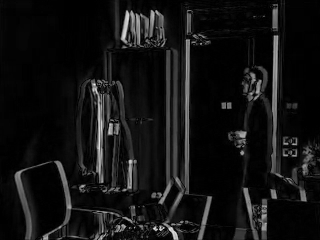
\includegraphics[width=1\textwidth]{../assets/images/04-diff-curr-prev-1.png}
        \caption{Absolute difference between current and previous frame}
        \label{fig:diff-curr-prev}
    \end{subfigure}
    \hfill
    \begin{subfigure}[b]{0.3\textwidth}
        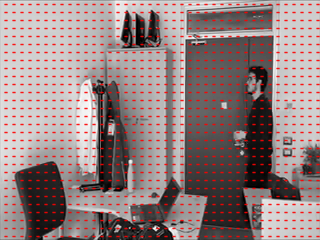
\includegraphics[width=1\textwidth]{../assets//images/04-camera-motion-1.png}
        \caption{Global motion field estimated by our procedure}
        \label{fig:est-mf}
    \end{subfigure}
    \hfill
    \begin{subfigure}[b]{0.3\textwidth}
        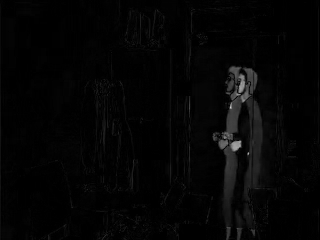
\includegraphics[width=1\textwidth]{../assets/images/04-diff-curr-comp.png}
        \caption{Absolute difference between current and compensated frame}
        \label{fig:diff-curr-comp}
    \end{subfigure}

    \caption{Estimated trajectories.}
\end{figure*}

\paragraph{How to interpret the results shown in \red{qualitative-result-image}} We should be able to notice in the results that the motion that we can register between the two frames is pretty large. In fact, we can see that a big part of the visual field seems to be moving in \red{ref second-row-position-1}.

However, if we compute the motion generated by the camera egomotion, we find out that most of the shift we record is apparent.
By estimating the motion generated by the camera, which is reported in  \red{ref second-row-position-2}, we can compensate the apparent motion in the previous frame.
When we compensate the previous frame we delete all the motion due to apparent motion and, therefore, if we compare the current frame and the compensated frame (see \red{ref second-row-position-3}) we are able to isolate real motion.

The results shown are consistent since the video from which the frames are taken was recorded with the camera moving in the horizontal direction while the person in the video was walking.

\subsection{Quantitative results}

To perform a numeric quantitative analysis of the results produced by the algorithm we used, once again, the compensation of the previous frame. Basically, in a video sequence where there is no real motion, but only camera motion, the compensation of the apparent motion should be enough tho make the current and the compensated frame identical.

Therefore, in \red{insert table}, we present some PSNR values for different video sequences. We annotated the table with some considerations about the videos, since PSNR value is influenced also about properties of the video like the strength of motion or the presence/absence of real motion.

\begin{table}
    \label{tab:psnr}
    \begin{tabular}{ll|rrrr}
    \toprule
    Video & Properties & Average & Variance & Maximum & Minimum \\
    \midrule
    {\small\texttt{pan240.mp4}} & {\small Fast motion} & \(22.724\)  & \(5.125\)  & \(27.802\) & \(17.981\)  \\

    {\small\texttt{coastguard\_qcif.mp4}} & 
        \begin{tabular}{@{}c@{}}{\small Two objects moving,}\\{\small background moving}\end{tabular}
    & \(22.733\)  & \(2.194\)  & \(26.875\) & \(15.158\)  \\
    
    {\small\texttt{foreman.mp4}} & 
        \begin{tabular}{@{}c@{}}{\small Big object moving,}\\{\small still background}\end{tabular}
        & \(19.677\)  & \(18.443\)  & \(30.436\) & \(11.746\)  \\
        
    {\small\texttt{numeri\_del\_piero.mp4}} & 
        \begin{tabular}{@{}c@{}}{\small Medium object moving,}\\{\small moving background}\end{tabular}
    & \(19.072\)  & \(13.642\)  & \(47.722\) & \(16.323\)  \\
    

    \bottomrule
\end{tabular}
    \caption{PSNR result on a vunch of samples}
\end{table}    
